\documentclass[18pt]{article}
\usepackage{graphicx}
\usepackage[utf8]{inputenc}
\title{\textbf{Assignment-1}}
\author{Chittepu Rutheesh Reddy \\
  cs21btech11014}
  \begin{document}
\maketitle{}

\section*{4b}

If the straight lines $3x- 5y = 7$ and $4x+ ay+ 9 = 0$ are perpendicular to one 
another, find the value of a.

\section*{Solution}
If two lines are perpendicular, then product of their slopes is -1.
\bigskip

   Let the slope of line 3x - 5y =7 be $m1=\frac{3}{5}$
 \bigskip
   
   Let the slope of line 4x+ay+9=0 be $m2=\frac{-4}{a}$ 
  \\
   
   As  \,\, m1m2 = -1
   \\ 
   
   ($\frac{3}{5}$)($\frac{-4}{a}$) = -1 
  \\
 
   So    $a = (\frac{12}{5})$ \\
  
  \graphicspath{{D:/Semester 2/Probability and Random Variables AI1110/Assignments/1/}}   
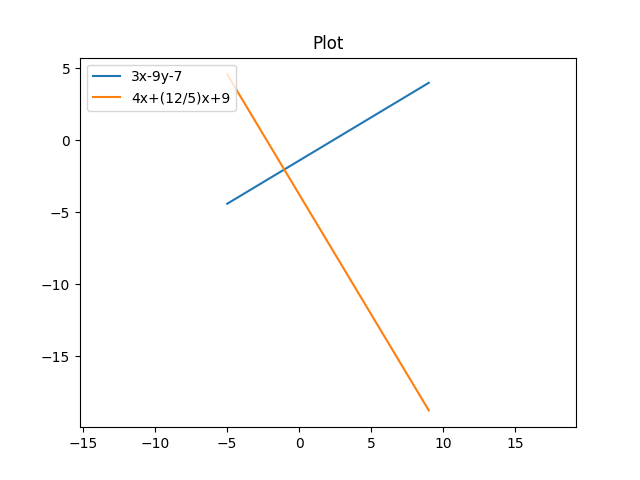
\includegraphics[scale=0.5]{Figure_1}

\end{document}